\chapter{Arquitecturas}\label{cha:arquitectura}

%El capítulo 2 describe la arquitectura de DuinoBot, Myro, Remotebot y
%XRemoteBot detallando las mejoras provistas por XRemoteBot.

% FIXME: QUIZAS ESTE CAPITULO PODRÍA IR ANTES DEL ANTERIOR... YA QUE SEGURAMENTE VAS A NOMBRAR Y DESCRIBIR VARIAS COSAS QUE LUEGO NOMBRAS ALLÁ... FIJATE

Tanto Remotebot como XRemoteBot tienen arquitecturas complejas que
dependen de otras librerías y de software instalado en los robots,
el objetivo de este capítulo es describir la interacción entre los
distintos dispositivos y aplicaciones utilizadas, demarcando el límite
entre el desarrollo realizado para esta tesina, XRemoteBot, con el software ya
existente con el que interactúa.

\section{Myro}\label{sec:myro}

Myro [REF] es la biblioteca utilizada para controlar a los robots ``Scribbler''
desde un script Python. Esta biblioteca puede interactuar con los robots de 2
formas diferentes: a través de un cable serial (RS323) o bien usando bluetooth
con RFCOMM. El funcionamiento de Myro requiere que el robot tenga
cargado un firmware determinado que espera las instrucciones desde el puerto
serial con el que cuenta el robot (el adaptador bluetooth se conecta en ese
mismo puerto serial).

\begin{figure}
    \centering
    \includegraphics[width=.7\textwidth]{figures/diagrama_myro}
    \caption{Diagrama de bloques de Myro}
    \label{fig:diagrama_myro}
\end{figure}

La figura~\ref{fig:diagrama_myro} muestra la interacción entre los componentes
más importantes de software y hardware desde el script del usuario hasta el
robot.

\section{DuinoBot}\label{sec:duinobot}

La biblioteca de Python
DuinoBot~\footnote{\url{https://github.com/Robots-Linti/duinobot}}
desarrollada en conjunto entre un grupo
de becarios del laboratorio LINTI de esta Facultad y la empresa RobotGroup
cuenta con un modo de operación similar al de Myro, conectándose con
los robots a través de un dongle XBee (que utiliza el protocolo ZigBee)
conectado a través de un puerto USB con el dispositivo controlante.
Para que esta biblioteca pueda controlar a los robots estos últimos
deberán tener instalado también un firmware especial: en este caso,
es un una versión modificada de un firmware que implementa el protocolo
Firmata de uso amplio para controlar dispositivos Arduino a través de una
interfaz serial que habitualmente es el puerto USB, pero en este caso
la interfaz serial está conectada a un dongle XBee en el robot, la interacción
entre las distintas capas de software y hardware se ilustra en la
figura~\ref{fig:funcionamiento_duinobot_diagrama}.

\begin{figure}
    \centering
    \begin{subfigure}[b]{0.7\textwidth}
        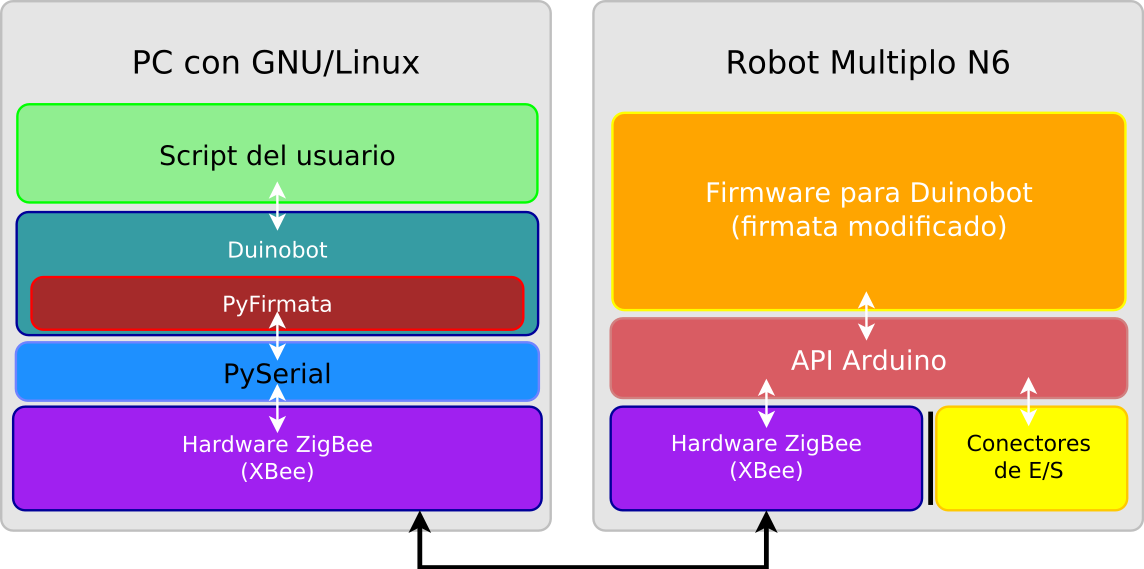
\includegraphics[width=.95\textwidth]{figures/diagrama_duinobot}
        \subcaption{Diagrama de bloques de DuinoBot}
        \label{fig:funcionamiento_duinobot_diagrama}
    \end{subfigure}
    \begin{subfigure}[b]{0.29\textwidth}
        \includegraphics[width=\textwidth]{figures/arquitectura_actual}
        \subcaption{Esquema de conexión típico}
        \label{fig:funcionamiento_duinobot_conexion}
    \end{subfigure}
    \caption{Funcionamiento de DuinoBot}
    \label{fig:funcionamiento_duinobot}
\end{figure}

La modalidad de uso esperada con DuinoBot consiste en que cada usuario
debe contar con una computadora, conectada por USB a un dongle XBee,
y desde esa computadora puede controlar uno o más robots. Con esa modalidad
fueron utilizados los robots en los cursos del proyecto
``Programando con robots y software libre'' y en actividades similares
planteadas posteriormente, generalmente además cada alumno controla
un único robot, el esquema de conexión típico en estos cursos se encuentra
ilustrado en la figura~\ref{fig:funcionamiento_duinobot_conexion}.

\section{Remotebot}\label{sec:remotebot}

La versión original de Remotebot fue presentada como trabajo práctico
de la materia Laboratorio de
Software~\footnote{\url{http://wiki.labmovil.linti.unlp.edu.ar/index.php?title=RemoteBot:_Android_\%2B_Robots}}
el objetivo principal del trabajo era desarrollar una aplicación para
dispositivos Android que accediera a sensores y posiblemente a la red
wireless usando el lenguaje Java.

% FIXME: REDACTAR MEJOR ESTE PARRAFO

Para este trabajo se implementó
RemoteBot4Android~\footnote{\url{https://github.com/fernandolopez/remotebot4Android}},
una aplicación Android
que permite controlar robots usando los acelerómetros de los dispositivos
móviles donde se ejecuta, inclinar el dispositivo en
una dirección provoca que el robot se mueva en esa dirección, además
esta aplicación cuenta con un indicador que muestra la distancia al obstáculo
más cercano sensado por el robot y una botonera para controlar al robot
sin usar los acelerómetros.

El producto principal de este trabajo fue el cliente
Remotebot4Android pero además del cliente, se desarrolló un 
protocolo de comunicaciones
y un servidor básico que atiende los requerimientos y se los envía al
robot correspondiente, respondiendo también a peticiones de datos de
los sensores del
robot, ésta fue la primer implementación del servidor
Remotebot~\footnote{\url{https://github.com/fernandolopez/remotebot}}
en cuyo concepto está basado XRemoteBot.

Remotebot provee una API JSON a través de HTTP que permite controlar a los
robots de forma remota, pero si bien es posible poner el servicio público,
el mismo no cuenta con autenticación, no soporta bien la concurrencia
y no provee ningún mecanismo de seguridad por lo que es recomendable solamente
usarlo dentro de ámbito de una red LAN.
La implementación del servidor
usa el módulo ``SimpleHTTPServer'' de la biblioteca estándar de Python para
proveer el soporte del protocolo HTTP e
introspección~\footnote{\url{http://www.ibm.com/developerworks/library/l-pyint/}}.
para convertir los
mensajes enviados por los clientes en invocaciones a métodos.

\begin{figure}
    \centering
    \begin{subfigure}[b]{0.78\textwidth}
        \includegraphics[width=.95\textwidth]{figures/diagrama_remotebot}
        \subcaption{Diagrama de bloques de Remotebot}
        \label{fig:diagrama_remotebot}
    \end{subfigure}
    \begin{subfigure}[b]{0.2\textwidth}
        \centering
        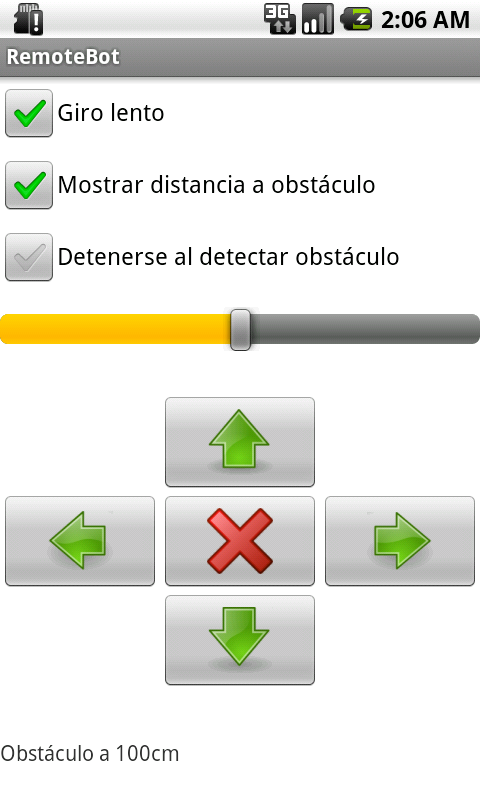
\includegraphics[width=\textwidth]{figures/cliente_remotebot}
        \subcaption{Cliente de Remotebot}
        \label{fig:cliente_remotebot}
    \end{subfigure}
    \caption{Diagrama de bloques e imagen del cliente Remotebot}
    \label{fig:diagrama_y_cliente_remotebot}
\end{figure}

Como se ve en la figura~\ref{fig:diagrama_remotebot} Remotebot utiliza la
biblioteca DuinoBot para comunicarse con los robots y el cliente para el cuál
fue diseñado es una aplicación Android que permite controlar los robots
y ver los valores del sensor de distancia usando una interfaz con botones,
además de poder controlar el robot usando los acelerómetros del dispositivo
(inclinar el dispositivo en una dirección dada hace que el robot se mueva
en esa dirección).

\section{XRemoteBot}\label{sec:xremotebot}

La interacción de XRemoteBot a nivel arquitectura es muy similar a la provista por Remotebot,
con la salvedad que el primero, además soporta robots Scribbler y puede ser
ampliado para interactuar con otros robots. Desde el punto de vista del cliente
XRemoteBot tiene varias diferencias, entre ellas la elección del protocolo,
usándose Websockets en lugar de peticiones HTTP y la definición del protocolo
de capa de aplicación que si bien es similar, ahora cuenta con un saludo y
un paso de autenticación a través de una ``API key''.



